\begin{figure*}[h] % two pictures
	\centering
	\begin{subfigure}[t]{0.47\linewidth}
		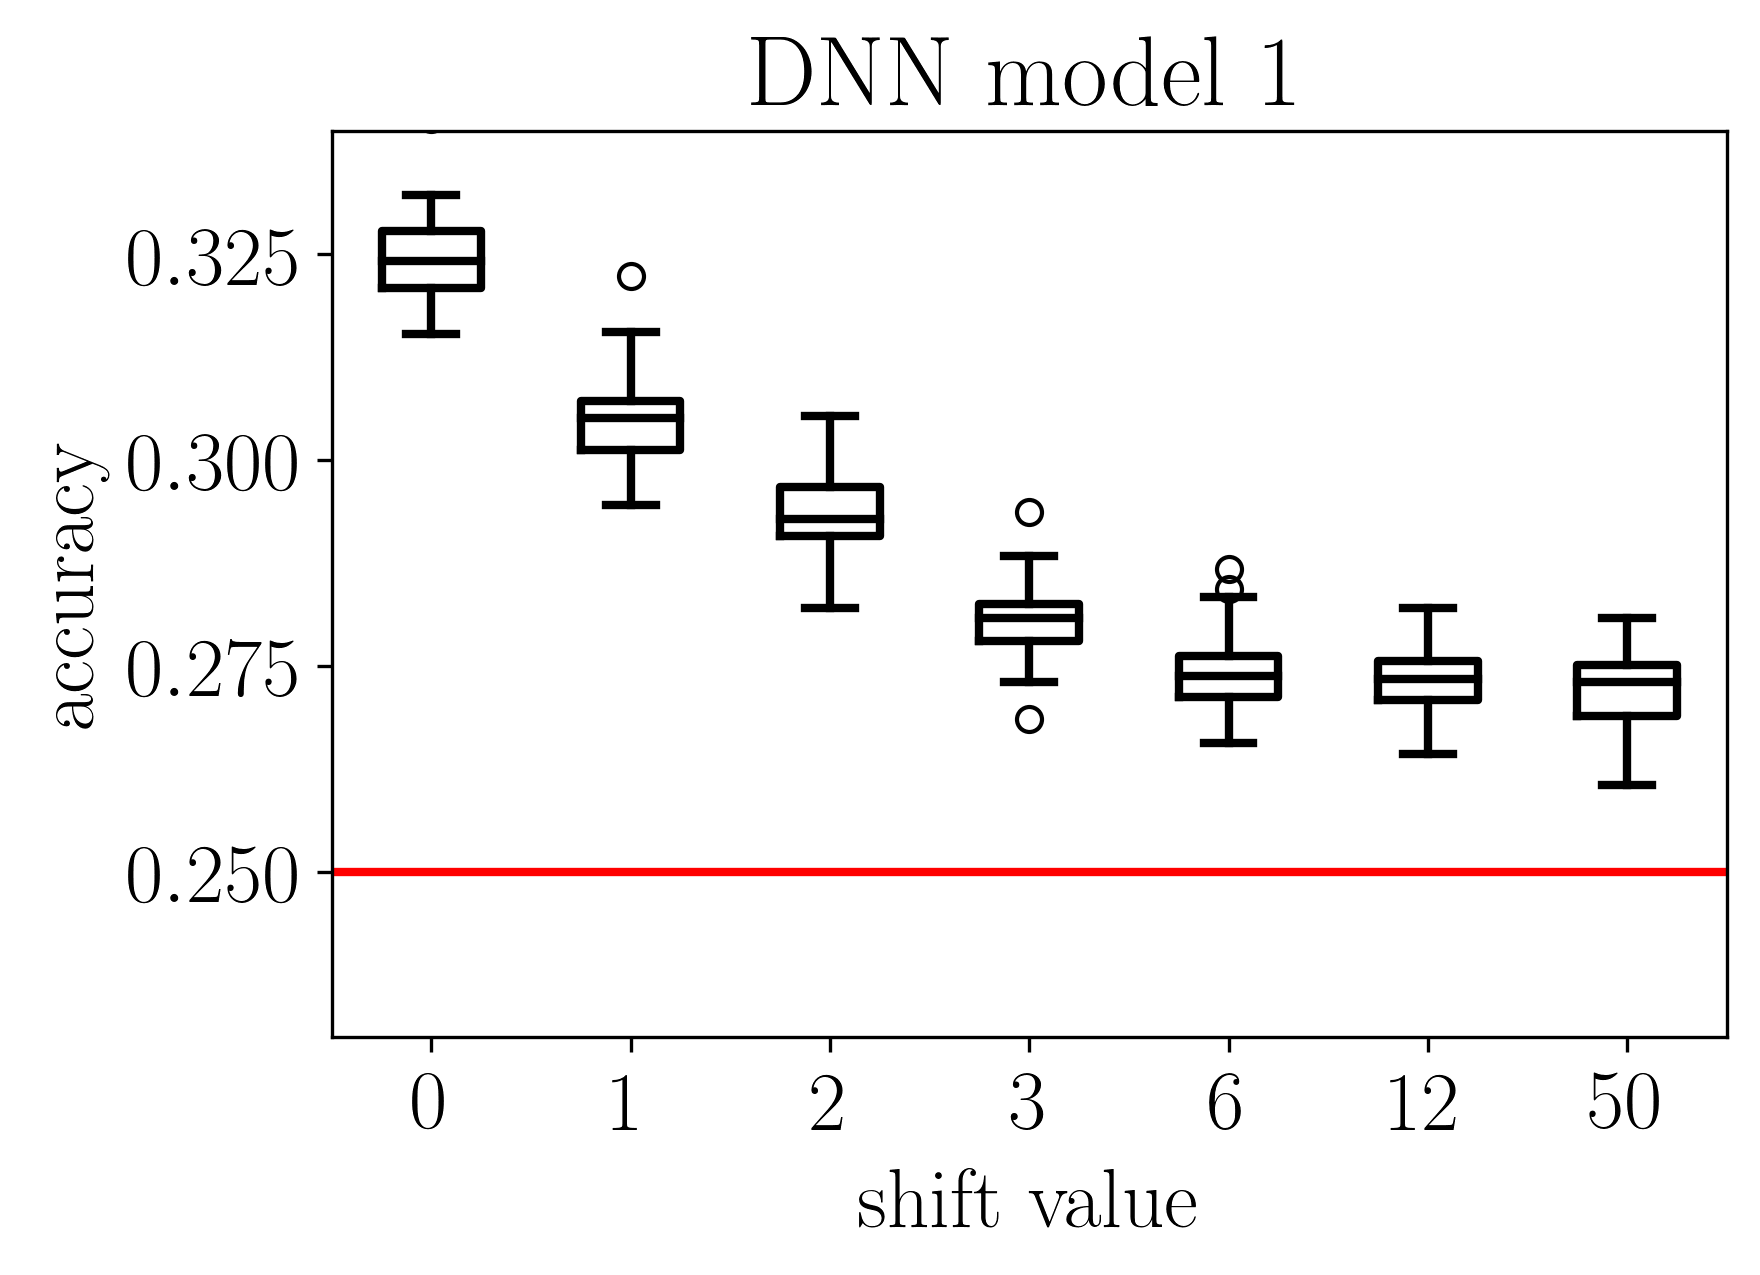
\includegraphics[width = \textwidth]{pics/dnn_model_1_all_runs_p1_ecoli_100000_10000_12_all.png}
		\caption{{\bfseries DNN model 1} \\*
		Полносвязная однослойная модель. Размер предикторной области 12.
		}
		\label{fig:dnn_shift}
	\end{subfigure}
	\begin{subfigure}[t]{0.47\linewidth}
		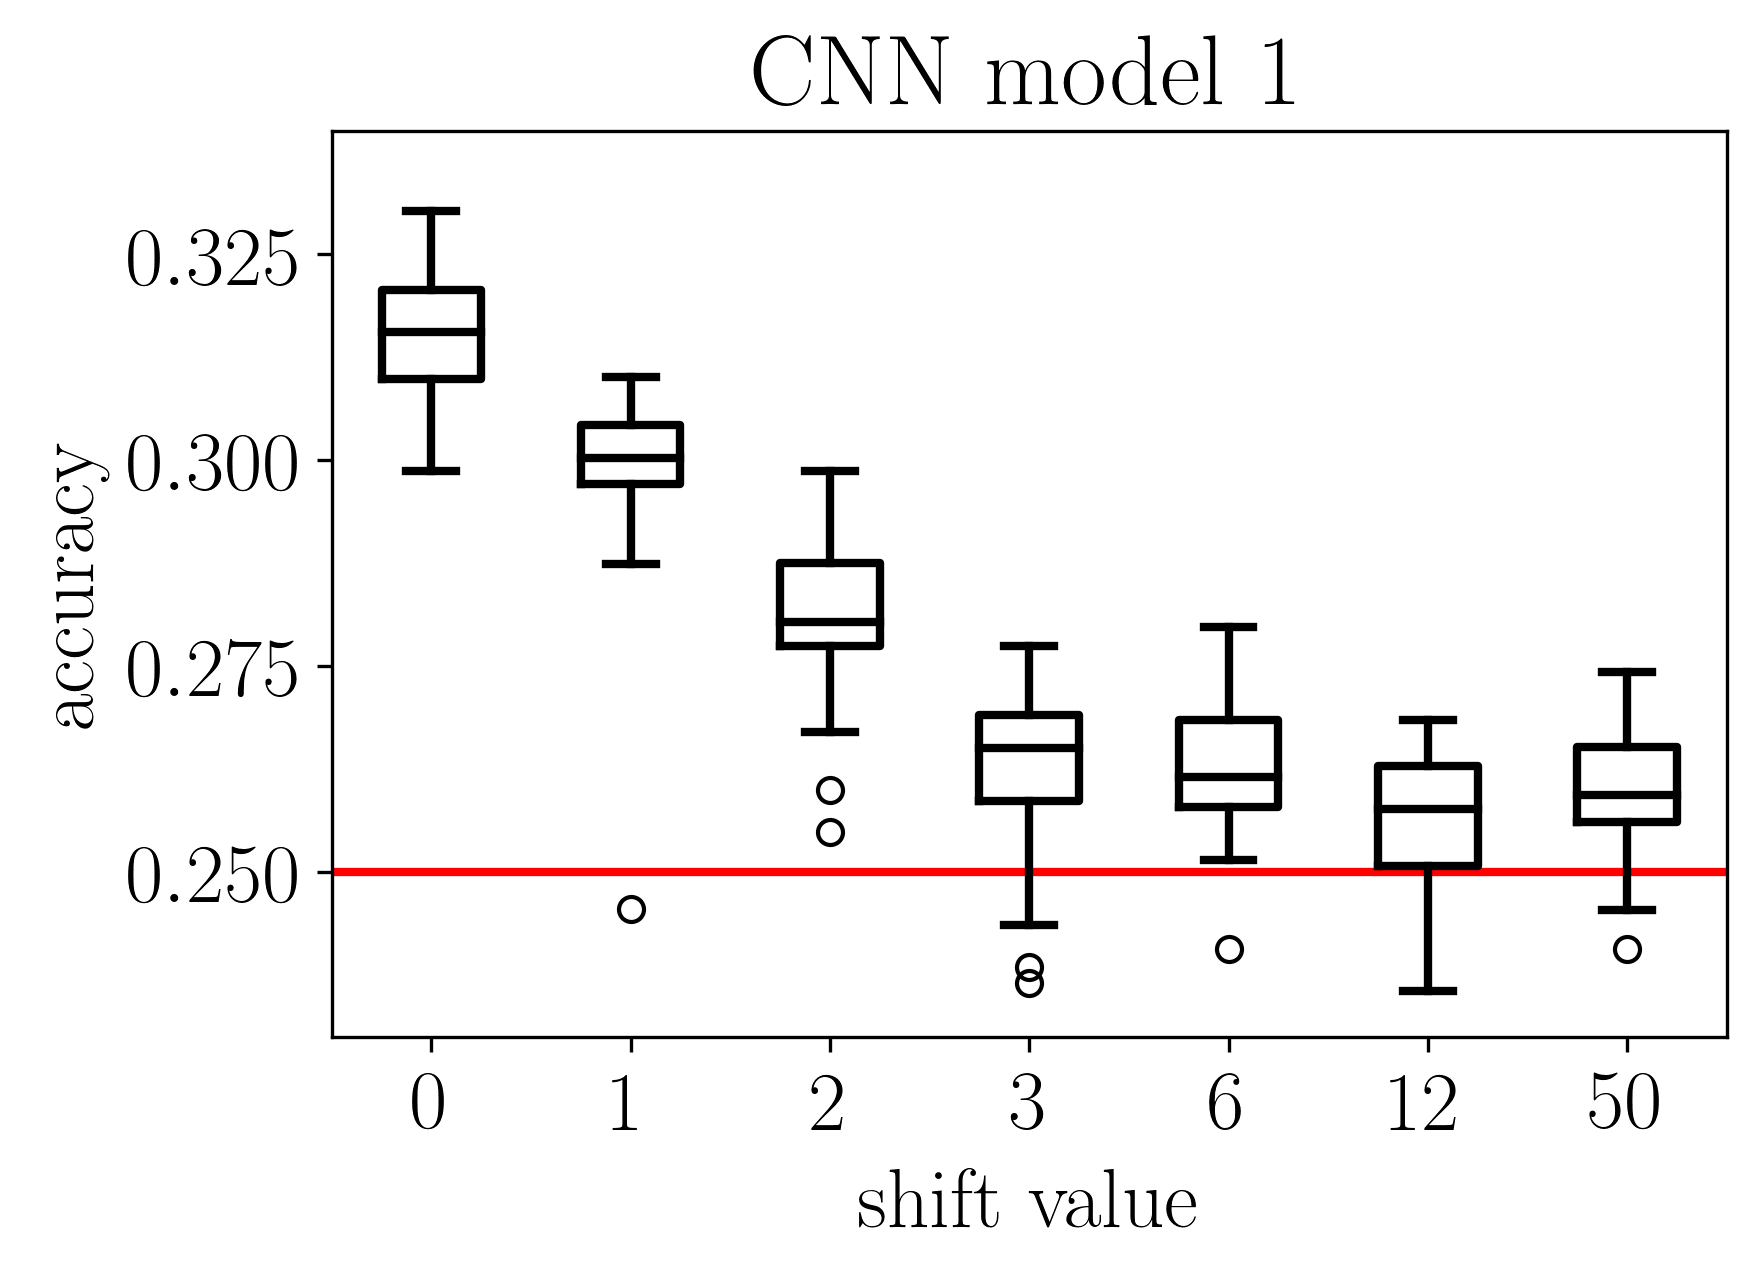
\includegraphics[width = \textwidth]{pics/cnn_model_1_all_runs_p1_ecoli_100000_10000_6_all.png}
		\caption{{\bfseries CNN model 1 (kernel = 3)} \\*
		Сверточная однослойная модель. Размер предикторной области 6.
		}
		\label{fig:cnn_shift}
	\end{subfigure}
	\caption{{\bfseries Зависимость точности предсказания от расстояния между предикторной областью и предсказываемым нуклеотидом (от отступа)  для различных архитектур.} \\*
	По горизонтальной оси обозначен размер отступа. По вертикальной оси показано распределение точностей обученной модели в 30 запусках с различными наборами данных. Горизонтальная линия отмечает точность случайного предсказания 25\%.}	
	\label{fig:shift}
	
\end{figure*}